\section{City-folding Visual Analytics}

Semantic understanding of social characteristics.

\subsection{Data-driven Profile Visualization}

Glyph-based visualization~\cite{borgo2013glyph} is the form of visual design to compose multivaribles into a collection of unified visual symbols, known as glyph. Glyph is intended for quick understanding and aligned comparison. Among glyph design, Chernoff Face~\cite{chernoff1973use} represents data variabules by the different features of a cartoon face. Following the idea of Chernoff Face~\cite{chernoff1973use}, we design a type of glyph, a graphical representation of people with specific demographic characteristics. The idea behind using faces is that humans easily recognize faces and notice small changes without difficulty. Those visual profiles are intended for intutive visual understanding and clustering, to abstract to concrete and semantic understanding, to help users clues to target the interested individual groups effectively.

Figure~\ref{fig:design_profile} shows the legend for the user profile. Those design dimensions are driven by data.The eight demographic dimensions are systematically designed into different visual symbols. Considering there are two types of variables, i.e., the numeric attributes and categorical attributes. By different composition, stimulus pattern which has the abstract deomgraphic measurement of individuals.

\begin{itemize}
\item \textbf{Gender} the gender is visually mapped to the hair style of the avatar. 
\item \textbf{Age} age is implied by the decoration on the hair. For the elder above 70, the hair is dyed to gray. For the youth beneath 18, hair decoration for girls and boys are adapted to the hair style.
\item \textbf{Education} The thickness of eye glasses is used to indicate the different levels in education.
\item \textbf{Job} The clothes is designed to imply the job of the individual. There are 9 types of clothes.
\item \textbf{Belongings} for house, car, residential license are considered as the belongings to the individual, so we design each of them as an add-on decoration to imply whether the individual has it or not.
\item \textbf{Income} a money symbol is used to show the different income levels.
\end{itemize} 

\begin{figure}[htb!]
 \centering % avoid the use of \begin{center}...\end{center} and use \centering instead (more compact)
 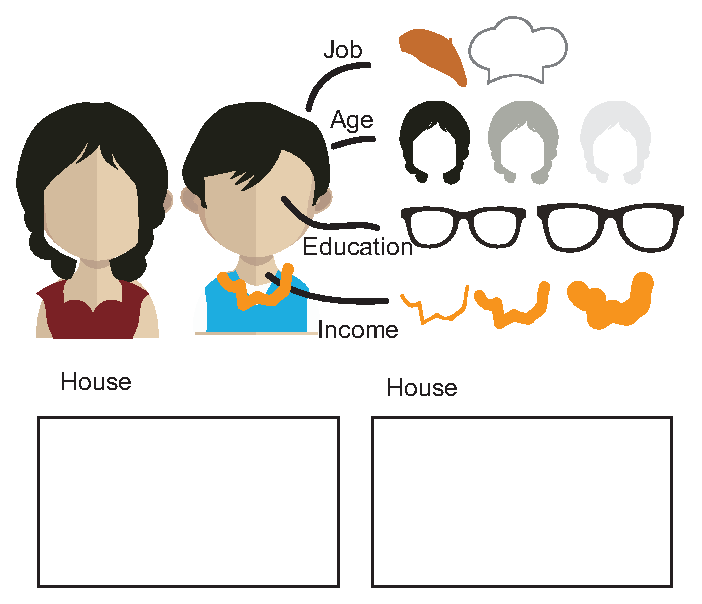
\includegraphics[width=\columnwidth]{pictures/design_profile}
 \caption{Design Profile}
 \label{fig:design_profile}
\end{figure}

With the visual mapping, the profiles varies from individual to individual. Figure~\ref{fig:div_profile} shows some examples. By concretizing the attributes which otherwise is too abstract to percept, users can scan and search for interesting target organically in figures.

\begin{figure}[htb!]
 \centering % avoid the use of \begin{center}...\end{center} and use \centering instead (more compact)
 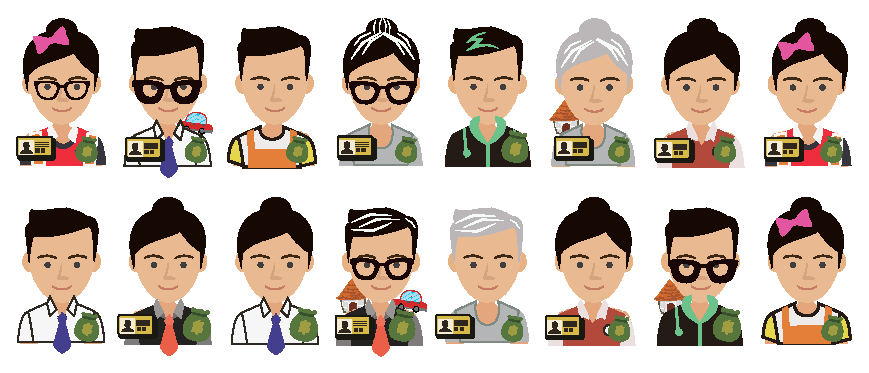
\includegraphics[width=\columnwidth]{pictures/design_div}
 \caption{Diverse Profile}
 \label{fig:div_profile}
\end{figure}

\subsection{T-SNE Projection}

Each individual is denoted as a vector with eight factors and projected as a dot into the 2D view by the T-SNE project~\cite{}. As 
Figure~\ref{fig:mds} shows, the whole space of volunteers are plotted evenly in the 2D view, which idnicates the uniformly sampled. Cross-filter~\cite{} from 

Classification Updated. Automatic ensembling of diverse profiles. 

Groups from demographics

\begin{figure}[htb!]
 \centering % avoid the use of \begin{center}...\end{center} and use \centering instead (more compact)
 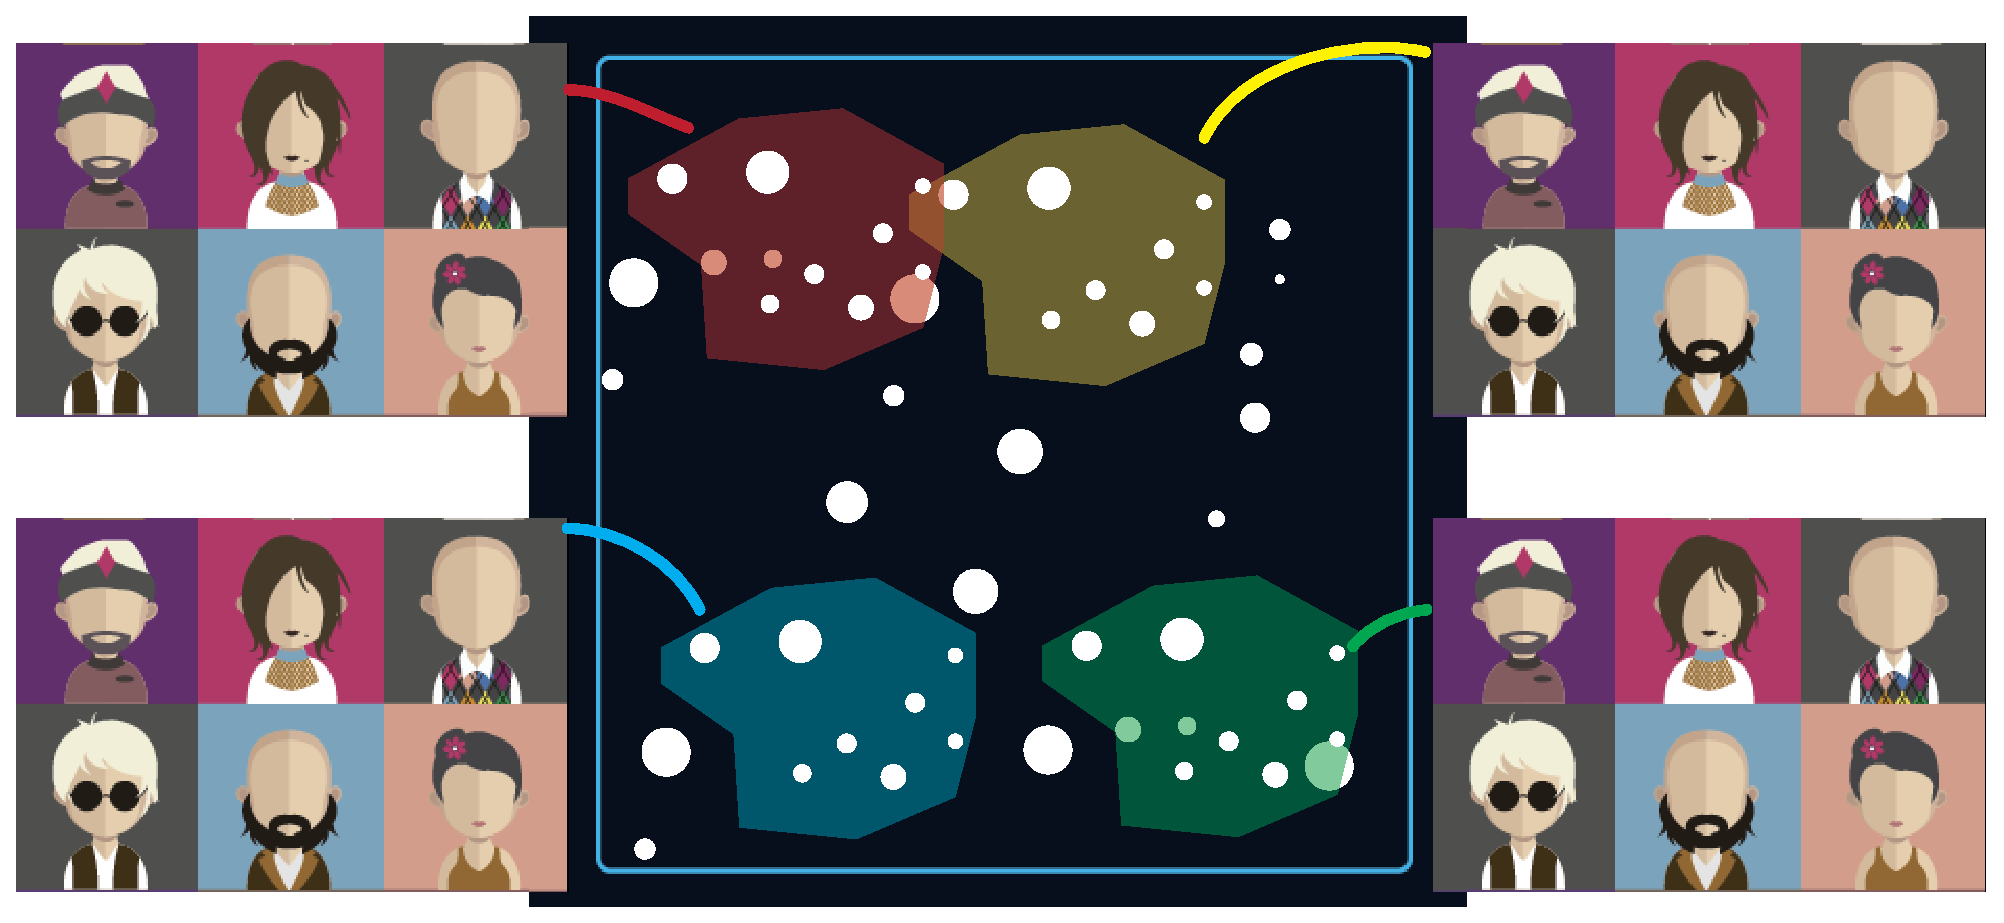
\includegraphics[width=\columnwidth]{pictures/mds}
 \caption{Interactive Labelling and Classification}
 \label{fig:mds}
\end{figure}

\subsection{2.5D Spatial Visualization}

The space visualization is embedded in 2.5D space. TAZ is used as the .... The height of space is put as the occurrence of visiting. For each group of people, we adjust the DB-Scan Algorithm in the context of TAZ. 

Travel Purpose, Clustering, Small Multiple Comparison